\ifdefined\TWOCOLUMN
    \documentclass[aps,prl,twocolumn,superscriptaddress,showpacs]{revtex4-2}
\else
    \documentclass[aps,prl,preprint,superscriptaddress,showpacs,endfloats]{revtex4-2}
\fi

\bibliographystyle{apsrev4-1}

\usepackage{bm}
\usepackage{amsmath,amssymb}
\usepackage{braket}
\usepackage{graphicx}
\usepackage{epstopdf}
\graphicspath{{./figures/}}
\usepackage{url}
\usepackage{textcase}
\usepackage{hyperref}

\ifdefined\LINENO
    \usepackage{lineno}
    \linenumbers
\fi

\def\vector#1{\mbox{\boldmath $#1$}}
\ifdefined\GITHASH
    \usepackage{fancyhdr}
    \pagestyle{fancy}
    \rhead{\GITHASH}
    \ifdefined\GITDATE
        \lhead{\GITDATE}
    \fi
    \ifdefined\GITBRANCH
        \chead{\GITBRANCH}
    \fi
\fi

\usepackage[utf8]{inputenc}
\usepackage[T1]{fontenc}

\begin{document}

\ifdefined\GITHASH
    \ifdefined\GITDATE
        \ifdefined\GITBRANCH
            \date{\GITDATE\ \#\GITHASH\ on\ \GITBRANCH}
        \else
            \date{\GITDATE\ \#\GITHASH}
        \fi
    \fi
\else
    \date{\today}
\fi

%TC:ignore
\title{Supplementary Information of Title}
\author{First Author}
\email{first@author.email}
\affiliation{First Author's Affiliation}
\author{Second Author}
\affiliation{Second Author's Affiliation}

\renewcommand{\thepage}{S\arabic{page}}
\renewcommand{\thefigure}{S\arabic{figure}}
\renewcommand{\thetable}{S\arabic{table}}
\renewcommand{\theequation}{S\arabic{equation}}

\flushbottom
\maketitle

\thispagestyle{empty}
%TC:endignore

\section*{Description 1}
Citing a reference\cite{example}.

In line equation: $e^{i\pi} + 1 = 0$.
Using equation environment:
\begin{equation}
    \hat{H}\Psi = i\hbar\frac{\partial}{\partial t}\Psi
    \label{eq:schroedinger_eq}
\end{equation}
and referring to it as Eq.~\ref{eq:schroedinger_eq}.

Showing a figure and referring to it as Fig.~\ref{fig:example_fig1}
%figure 1
\begin{figure}
    \caption{
    Example supplementary figure 1.
    }
    \label{fig:example_fig1}
    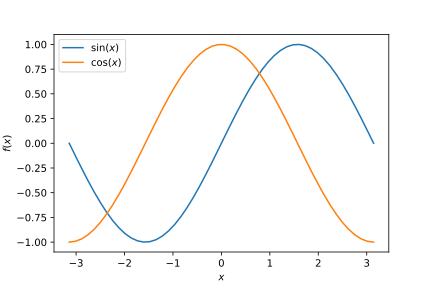
\includegraphics[width=\linewidth]{example_fig1.pdf}
\end{figure}

Showing a table and referring to it as Table~\ref{table:example_table1}.
%table 1
\begin{table}
    \caption{
        Example supplementary Table 1.
    }
    \label{table:example_table1}
    \centering
    \begin{tabular}{ccc}
       a & b & c \\
       \hline
       1 & 2 & 3 \\
    \end{tabular}
\end{table}

\bibliography{./references}
\end{document}
